\chapter{Analog Foundation of Digital Circuits}
\label{chapter:Analog Foundation}
\graphicspath{ {./chapter09/Fig} }

One of the greatest skills in a computer engineers repertoire 
is their skill with electrical concepts.  Happily, a few 
key concepts are sufficient to guide you
through even the most technical assignment.  In this chapter 
you will be introduced to the analog aspect of basic gates
introduced in chapter 2.  

%\section{Prerequisite Concepts}
%\subsection{Voltage Sources}
%\subsection{Thevenin Equivalence}
%\subsection{RC delay}
%\subsection{Transistors}
%\section{Logic Families}
%\subsection{TTL}
%\subsection{CMOS}


The nomenclature used to identify basic gates  is
composed of three pieces.  In order these are grade, technology and
device.  There are two grades of devices, 74 series are commercial
grade and 54 series are military grade.  The difference has to do 
with the amount of in-house testing that is done to the device before
it leaves the factory.  Since military grade components spend more 
time undergoing testing, hence you will
probably find 74 series devices in your university electronics
lab.  A chip's technology refers to the process used in the transistor
level design and fabrication processes used to construct the chip.
Two of the most common technologies are the LS and HC.  LS technology 
is often referred to as TTL and the HC technology is referred to as 
CMOS.  Only if you are looking for very specific device characteristics
do you need to worry about the technology.  Otherwise the trade offs 
between these two two technologies results in either being a fine 
choice for most university projects.  The final part of a 
devices identification is its number.  Commonly used parts have two 
digit designations, like the 00 and 32.  Three and four digit parts 
like a 373 and 4722 represent esoteric parts which generally are hard 
to find and costly.

\section{Data Sheet}
The complete specification of any basic gate is described in its
associated data sheet.  For the subsequent discussion you
will need to locate the data sheet on page~\pageref{page:74ls00} 
describing a 74LS00 quadruple 2-input nand gate.
The data on a data sheet can be overwhelming at first.  However lets
takes it one page at a time and discuss what we see along the way.

%% \subsection{Page 1}
The first page describes the devices behavior.  The text under
the \textbf{ description} heading tells it all,
\begin{quote}
	"These devices contain four independent 2-input NAND gates."
\end{quote}
On the right side, the data sheet shows the three possible
chips packages that you can purchase.
Generally you will find J packages in university labs, the other two
begin relegated to special purpose industrial/military applications.
Once you have located the picture of the 74LS00 J package you should
note the names and order of the labels associated with the pins.  Like
most common household electronic devices, these gates require an
independent source of power.  On most digital circuits the \VCC pin
is attached to 5 volts and $GND$ is attached to 0 volts.  The remaining
pins can be divided onto four groups according to their number.  Each
number has three associated pins, for example, 2A, 2B and 2Y.  These
letters are used in the truth table description of the circuit relating the
inputs A,B to the output Y.  Up to this point there should be no surprises
so lets flip to page 2 of the 74ls00 data sheet.

%% \subsection{Page 2}
Page 2 is a smorgasbord of transistors and other discrete components.
This page will become important later when we discuss open collector 
outputs, but for the time being we will skip all the schematics and 
turn to page 3 of the 74ls00 data sheet.


%% \subsection{Page 3+}
Congratulations, you made it to the end of the data sheet!  This is the
real meat-and-potatoes section.  Most logic devices, be they
FPGAs or PALs will have a page listing the recommended operating conditions,
electrical characteristics and switching characteristics.  Lets walk
through this third page from top to bottom starting with the 
\textbf{ recommended operating conditions} section.  
A portion of the recommended operating conditions table is duplicated
below with an additional figure to the right showing the I/O values
relevant to the listed parameter as well as an equivalent circuit 
superimposed on the nand gate describing its analog behavior for
the listed parameter.

\begin{tabular}{l|l|lll|l||l}
Name& Definition		& Min & Nom & Max & units & Equivlent Circuit 	\\ \hline
\VCC & Supply Voltage		& 4.75& 5   & 5.25& V     &	\\ \hline
\VIH & High-level input voltage	& 2   &     &     & V     &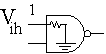
\includegraphics{vih} \\ \hline
\VIL & Low-level input voltage	&     &     & 0.8 & V     &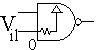
\includegraphics{vil} \\ \hline
\IOH & High-level output current&     &     &-1.0 & mA    &
\includegraphics{ioh} \\ \hline
\IOL & Low-level output current	&     &     &20.0 & mA    &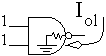
\includegraphics{iol} \\ 
\end{tabular}

Starting at the top of the table
the \VCC measurement just describes the supply voltage that the device will
tolerate on a continued basis.  If the \VCC and GND are reversed the
chip will get so hot that it will start to melt.  Your sense of smell and 
judicious touching of chips is debugging tool frequently used early in a 
circuits development.  \VIH is the smallest voltage which is recognized by 
the input as a logic 1.  Its important to note this value is a minimum, 
clearly any larger value should also be recognized as a logic 1.  The 
equivalent circuit show that the input voltage is dropped across a resistor
to ground.  This resistor forms the input impedance of the nand gate and
is typically around a mega ohm.  \VIL is the maximum voltage which is 
recognized as a logic 0.  \IOH is the maximum current that an output can 
supply.  The Thevenin's equivalent of the output shows that current flows 
out of the output because it comes from \VCC.
\IOL is the maximum amount of current that can flow into the nand gate
output when the output is low.  It may seem counterintuitive that current flows
into an output but the equivalent circuit shows that by pulling the output
low the Thevenin's equivalent output is a resistor tied to ground.  It
should be clear from the Thevenin's equivalent circuit that current flows
to ground, hence into the output of the nand gate.

The next table on page 3 is titled 
\textbf{ electrical characteristics over recommended operating free-air
temperature range}.  As before select rows will be accompanied by
a figure describing the electrical behavior of the gate for the 
specified parameter.

\begin{tabular}{l|l|lll|l||l}
Name& Definition		& Min & Nom & Max & units &  	\\ \hline
\VOH & High-level output voltage& 2.7 & 3.4 &     & V     &
\includegraphics{voh} \\ \hline
\VOL & Low-level output voltage	&     &     & 0.5 & V     &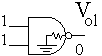
\includegraphics{vol} \\ \hline
\IIH & High-level input  current&     &     & 0.05& mA    &
\includegraphics{iih} \\ \hline
\IIL & Low-level input  current	&     &     &-2.0 & mA    &
\includegraphics{iil} \\
\end{tabular}

\VOH is the minimum voltage that a nand gate will produce as a 
logic 1.  Typically, the output of a nand gate is very close to 5V, 
but it can drop lower when the output is heavily loaded.  \VOL is the
highest voltage a nand gate will output in the guise of logic 0.
Typically, a logic 0 output is close to ground but can increase if
a lot of current is dumped into the output (see \IOL above).  \IIL is
the maximum amount of current consumed by the nand gate when a logic
0 is applied to the input.  Its somewhat counter intuitive to think
about current flowing out of an input.  However the equivalent circuit
shows that the input is attached to \VCC consequently current flows
out of the input.  \IIH is the amount current consumed by an input
then a logic 1 is applied to an input.  The equivalent circuit shows
the input dropping to GND.

There are two important device parameters that can be calculated 
from the first two tables, fan-out and noise margins.  Both parameters
as based on the assumption that the nand gate will be used in a cascade
configuration; \index{cascade configuration|(} the output of a nand 
gate is the input to other nand gate(s).  Figure~\ref{fig:cascade} 
shows three cascaded nand gates.  From this figure it should be clear
that the nand gate in the middle of the cascade has its inputs
supplied by nand gates and deliver its output to nand gates.  Since
most of the 74LS series devices have similar electrical 
characteristics the notion of a cascade 
configuration is relaxed to mean that the inputs and outputs of a
74ls devices come from and go to other 74LS type devices.

\begin{figure}[ht]
\center{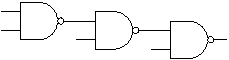
\includegraphics{cascade}}
\caption{A cascade sequence of nand gates.}
\label{fig:cascade_conf}
\end{figure}

\section{Noise Margin}
\index{noise margin|(}
In the real world the output of a device like our nand gate is subject
to electrical interference.  One of the most common forms of interference 
is a real or apparent disturbance in the voltage level at the output of a 
logic gate.  Such a disturbance can be viewed as adding a noise signal to
the intended logic voltage.  The noise margin of the nand gates in 
Figure~\ref{fig:cascade_conf} is the maximum amount of voltage that can 
be added to the output of nand gate A while still transmitting the 
intended logic value to the input of nand gate B.  There is a noise 
margin associated with each intended logic value; 0 and 1.  Lets 
start by examining the noise margin associated with logic
1.  The lowest voltage output by nand gate A for logic 1 is \VOH=2.7
volts.  The lowest voltage recognized as logic 1 by 
nand gate B is \VIH=2V.  Consequently, the high noise margin is the 0.7 
volts because that's how much voltage can be added to the output of
nand gate A while still maintaining a logic 1 at the input of nand gate
B. A similar argument can be seen to determine that the noise
margin associated with logic 0 is \VIL-\VOL=0.8-0.5=0.3.  If a
single value is required for the noise margin then it should be
the based on the most pessimistic assumptions; in our case the  
logic 0 noise margin of 0.3V.


\section{Fan Out}
\index{fan out|(}
It should be clear from your previous studies of digital circuits 
that an output of a logic gate may be connected to many inputs.  For
example, the output of a NOT gate in the \SOPmin realization of a 
function is usually connected to many AND gates.  The fan-out of an 
output is the number of distinct inputs it connects to.  When 
designing a real circuit there is a maximum fan-out
resulting from current consumed by the inputs and the current generated
by an output.  The maximum fan-out occurs when the total current demanded
by all the inputs is equal to the current supplied by a single input.  
Since the amount of current consumed by an input and generated by an
output depends on the logic level then a fan-out calculation must
be performed for both logic levels.  For the high logic level a nand
gate produces \IOH = 1mA, while each receiving nand gate consumes
\IIH = 0.05mA.  Hence, the logic 1 fan out is \IOH / \IIH = 1mA/0.05mA = 20.
Note, that the sign of the current is ignored because the sense of the 
current directions is consistent with
the output producing current and the inputs consuming current.  The fan-out 
associated with logic 0 is \IOL / \IIL = 20A/2mA = 10.  Again the signs
of the current are ignored because the output is consuming current and the
inputs are generating current.  If a single value for the fan-out 
is required is should be based on the smaller of the logic 1 and logic 0
constrained values.  In the case of our nand gate this means that 
the fan-out is equal to 10.


\section{I/O Impedance}
Digital devices are given very specific characteristics which make them
easy to work with.  Two important characteristics which are
generally given little attention are the input and output impedance.
Fundamental to any discussion of impedance is the concept of the
Thevenin's equivalence of an output.  Thevenin stated that an output
can be consider to be a voltage source in series with an impedance.
Likewise the input of a digital circuit can be modeled as an
impedance connected to \VCC or GND.  Figure~\ref{fig:impedance} shows 
these two abstractions on top of a pair of cascaded nand gates where
the nand gate to the left is trying to transmit logic 1 to the
nand gate to the right.

\begin{figure}[ht]
\center{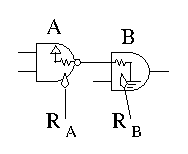
\includegraphics{impedance}}
\caption{The Thevenin's equivalence of an nand gates output feeding the
input impedance of a nand gate.}
\label{fig:impedance}
\end{figure}

The observations up to this point have been fairly straightforward.
We will now turn to investigate the relative values of the circuit
elements in Figure~\ref{fig:impedance}.  The whole point of the
circuit is to communicate the voltage generated by nand gate A to
nand gate B.  The two resistors in the equivalent circuit form the
well known voltage divider.  Hence, the voltage seen at the input
of the nand gate is 

	$$ \text{ V}_\text{ CC}  *
		\text{ R}_\text{ b}  / 
		( \text{ R}_\text{ a} + \text{ R}_\text{ b} ) $$


There are three
cases for the magnitude of \Ra and \Rb.  If \Ra were much larger
than \Rb then the \Rb/(\Ra+\Rb) would be a number less than 1 
and close to 0.  Hence, little of the nand gate A's voltage 
would reach the input of nand gate B.  Consequently, the input
to nand gate B may fall below \VIL and be interpreted as a logic
0.  Clearly, this is not
what want.  If \Ra were equal to \Rb then the ratio \Rb/(\Ra+\Rb) 
would equal 1/2, meaning that 1/2 of the voltage generated by nand
gate A would be seen at nand gate B.  While better than the first
case this still seems inefficient.  In the third case let
\Ra be much smaller than \Rb.  In this case the ration \Rb/(\Ra+\Rb)
is less than but close to 1.  Hence a majority of the voltage
generated by the nand gate A would be seen at the input of nand gate
B. This is just what we want, hence we arrive at the following
rule. \textit{ Generally, digital devices are built with small output
impedance and large input impedance so that the signal
generated by a source is dropped across the destination}.

\section{Open Collector}
Most digital circuits have active outputs.  This means that they drive 
their outputs to \VCC or to GND.  This is usually accomplished 
by a pair of transistors located at the output of the device.  The 
actual circuit is shown on page 2 of the 74ls00 data sheet,
a simplified view is shown in Figure~\ref{fig:transistor}.  To 
understand the behavior of this output you can consider 
a transistors as a switch.  When the base is at logic 1 there is
a short circuit between the collector and emitter.  When the base is 
at logic 0 there is an open circuit between the emitter and
collector.  With this very simplified model of a transistor in mind,
the operation of the nand gates outputs is greatly simplified.  In
order to drive the output $y$ to logic 0, the base of the lower 
transistor must be driven to logic 1 and the base of the upper
transistor must be driven to logic 0.  Thus, the output $y$ is then
connected directly to ground forcing the output to logic 0.  In order
to force the output to logic 1 the values on both bases are inverted.

\begin{figure}[ht]
\center{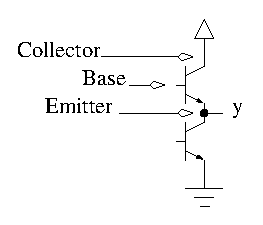
\includegraphics{transistor}}
\caption{A simplified 74ls00 output with the terminals of the 
transistor labeled.}
\label{fig:transistor}
\end{figure}

A digital circuit with an open collector output is missing the upper
transistor.  This means that the output can be connected to ground
but cannot be connected to \VCC.  In order to make an open collector
output operate properly, the output line must be tied to \VCC via
a resistor; typically 5k$\Omega$.

